
\begin{figure}
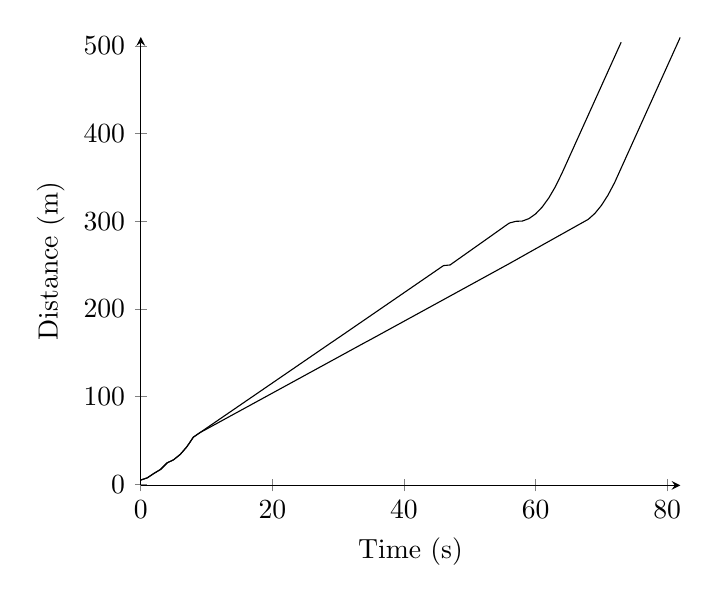
\begin{tikzpicture}
\begin{axis}[
legend style={anchor=west},
axis x line=bottom,
axis y line=left,
ymin=-1,
xlabel=Time (s),
ylabel=Distance (m),
]
\addplot[] coordinates {
(0, 5.1)
(1, 7.6)
(2, 12.6)
(3, 17.1)
(4, 24.5922199804)
(5, 28.1908323924)
(6, 34.2894448043)
(7, 42.8880572163)
(8, 53.9866696282)
(9, 59.0852820402)
(10, 63.1793368133)
(11, 67.2735453407)
(12, 71.3679153694)
(13, 75.4624551763)
(14, 79.5571736137)
(15, 83.6520801608)
(16, 87.7471849799)
(17, 91.8424989791)
(18, 95.9380338822)
(19, 100.033802306)
(20, 104.129817849)
(21, 108.226095185)
(22, 112.322650174)
(23, 116.419499988)
(24, 120.516663241)
(25, 124.614160153)
(26, 128.712012721)
(27, 132.810244922)
(28, 136.908882939)
(29, 141.007955422)
(30, 145.107493786)
(31, 149.207532555)
(32, 153.308109752)
(33, 157.40926736)
(34, 161.511051847)
(35, 165.513514785)
(36, 169.616408418)
(37, 173.719468428)
(38, 177.822709736)
(39, 181.926149103)
(40, 186.029805427)
(41, 190.133700095)
(42, 194.237857404)
(43, 198.342305077)
(44, 202.447074893)
(45, 206.552203456)
(46, 210.657733147)
(47, 214.763713319)
(48, 218.870201797)
(49, 222.97726678)
(50, 227.08498929)
(51, 231.193466351)
(52, 235.302815158)
(53, 239.413178645)
(54, 243.524733008)
(55, 247.637698049)
(56, 251.752351679)
(57, 255.934340867)
(58, 260.179579891)
(59, 264.395258762)
(60, 268.612266426)
(61, 272.831002226)
(62, 277.02454463)
(63, 281.218322931)
(64, 285.412441778)
(65, 289.607082495)
(66, 293.802596303)
(67, 297.99980209)
(68, 302.20154814)
(69, 308.90329419)
(70, 318.10504024)
(71, 329.80678629)
(72, 344.00853234)
(73, 360.60853234)
(74, 377.20853234)
(75, 393.80853234)
(76, 410.40853234)
(77, 427.00853234)
(78, 443.60853234)
(79, 460.20853234)
(80, 476.80853234)
(81, 493.40853234)
(82, 510.00853234)
};
\addplot[] coordinates {
(0, 5.1)
(1, 7.6)
(2, 12.6)
(3, 17.1)
(4, 24.5922199804)
(5, 28.1908323924)
(6, 34.2894448043)
(7, 42.8880572163)
(8, 53.9866696282)
(9, 59.124921206)
(10, 64.2634027598)
(11, 69.4021286962)
(12, 74.5411146514)
(13, 79.6803776253)
(14, 84.8199361336)
(15, 89.9598103808)
(16, 95.1000224571)
(17, 100.240596564)
(18, 105.381559273)
(19, 110.522939824)
(20, 115.664770465)
(21, 120.807086857)
(22, 125.949928531)
(23, 131.093339432)
(24, 136.237368553)
(25, 141.38207068)
(26, 146.527507278)
(27, 151.673747542)
(28, 156.820869648)
(29, 161.968962271)
(30, 167.018126401)
(31, 172.167809136)
(32, 177.317766387)
(33, 182.468030056)
(34, 187.618637195)
(35, 192.769631091)
(36, 197.921062645)
(37, 203.072992118)
(38, 208.225491397)
(39, 213.378646953)
(40, 218.532563739)
(41, 223.68737044)
(42, 228.843226601)
(43, 234.00033252)
(44, 239.158943227)
(45, 244.319388672)
(46, 249.482103647)
(47, 250.187673426)
(48, 255.518179143)
(49, 260.812751563)
(50, 266.109495352)
(51, 271.409287434)
(52, 276.713565624)
(53, 282.024883968)
(54, 287.348341439)
(55, 292.696278153)
(56, 297.960587371)
(57, 299.942626681)
(58, 300.261525306)
(59, 303.08042393)
(60, 308.399322554)
(61, 316.218221179)
(62, 326.537119803)
(63, 339.356018428)
(64, 354.674917052)
(65, 371.274917052)
(66, 387.874917052)
(67, 404.474917052)
(68, 421.074917052)
(69, 437.674917052)
(70, 454.274917052)
(71, 470.874917052)
(72, 487.474917052)
(73, 504.074917052)
};

\end{axis}
\end{tikzpicture}
\label{tik:distance:100:38}
\caption{100 percent diving with GSC on route $38$}
\end{figure}
